\documentclass[conference]{IEEEtran}
\IEEEoverridecommandlockouts
% The preceding line is only needed to identify funding in the first footnote. If that is unneeded, please comment it out.
\usepackage{cite}
\usepackage{amsmath,amssymb,amsfonts}
\usepackage{algorithmic}
\usepackage{graphicx}
\usepackage{textcomp}
\usepackage{xcolor}
\usepackage{comment}

\def\BibTeX{{\rm B\kern-.05em{\sc i\kern-.025em b}\kern-.08em
    T\kern-.1667em\lower.7ex\hbox{E}\kern-.125emX}}
\begin{document}

\title{Technology Platforms to Support Cancer Telerehabilitation: A Literature Review }

\author{\IEEEauthorblockN{Jose Andrés Mejías Rojas}
\IEEEauthorblockA{\textit{Universidad de Costa Rica}\\San José, Costa Rica\\
jose.mejiasrojas@ucr.ac.cr}}

\maketitle

\begin{abstract}
The objective of this literature review is to determine the characteristics of eHeath platforms for breast cancer patients. We aimed for fours aspects: the main features of the platforms, how were implemented, how were evaluated, and the usability and rehabilitation problems that were reported. We found out that most of the literature reviews are related to mobile apps. So we want to review every platform no matter if it's a mobile app or not. Moreover, we included the entire spectrum to determine whether the are lacks of relevant information.

We used three sources to do the literature review: ScienceDirect, Scopus, and JMIR Publications. The inclusion criteria was: studies between 2015 and 2021, primary investigations, reviewed by peers, eHealth related, and a case study or a study of an existent platform for breast cancer patients. Regarding the exclusion criteria, we defined three: English, omitting duplicated studies, and full access to the papers. We use PRISMA as the framework to perform the review.

We gathered 16 studies after the inclusion-exclusion review. We identified that the most popular feature is Recommendations/Learning. The majority of the platforms are mobile apps, and almost every study doesn't record technical decisions. Questionnaires are the most popular way to evaluate eHealth platforms, however, there isn't standardization. Finally, there are a variety of problems reported, so it was impossible to group them together. We concluded that informing patients about the cancer, therapies, diets, among others are important in eHealth platforms. Also, there is a need of guidelines to implement those kind of platforms, and standardization to evaluate them. Lastly, there is a lack of information related to technical decisions.
\end{abstract}

%\begin{IEEEkeywords}
%component, formatting, style, styling, insert
%\end{IEEEkeywords}

% Describa por qué el estudio es importante, qué lo diferencia de estudios existentes y cuál es el aporte que la revisión de literatura tendría para su posible tesis o TFIA.
\section{Introduction}
Humanity has been facing a war against cancer over the years. People already know how terrible the consequences are. Furthermore, there is a specific cancer that women in particular have been struggling: breast cancer. The battle against breast cancer has been complicated and, unfortunately, in some cases mortal \cite{burbank_knowledge_2006}. Cancer survivors need to decrease the side effects of surgery, so there is a need of good rehabilitation to improve their daily life and get back to normal \cite{de_rezende_telerehabilitation_2021}. However, humanity encountered an obstacle in 2020: COVID-19. Unfortunately, this pandemic has been forcing people to stay home as long as they can, wear masks on public places, and work from home. Cancer survivors are not an exception.

Telerehabilitation started to play a crucial role in this situation. Telerehabilitation is a subspecialty of telehealth that uses technologies to provide treatments \cite{galiano-castillo_agreement_2014, van_der_linden_feasibility_2018}. Patients follow a strict medical advice such as medication or therapy sessions.  

This paper explains the protocol and results of a literature review to gather information related to telerehabilitation of breast cancer. The purpose of this review is to seek out needs concerning technology platforms that support this subspecialty.

There are some systematic reviews related to eHealth. Kapoor et al \cite{kapoor_mobile_2020} made a systematic review to assess the availability and features of free mobiles apps for breast cancer survivors. Kumar et al \cite{kumar_mobile_2021} provided an overview of mobile and wearable sensing frameworks for mHealth. Finally, Jongerius et al \cite{jongerius_research-tested_2019} provided an overview of research-tested interventions using mHealth apps. As you can see, the majority of the systematic reviews are related to mobile apps.


Therefore, the difference between this study and other papers is that we looked for the entire spectrum like how the platforms were evaluated, what were the main features, what problems the platforms faced, and what were the crucial decisions to implement the respective platform. We included every platform available, so we didn't limit it to mobile apps exclusively. Hence, this paper will facilitate future work that may explore specific aspects the review helps to pop up.

\section{Review}

\subsection{Planning the Review}

% Objetivos o preguntas a contestar
\subsubsection{Research Questions} \label{subsubsection:research_question}
% ¿Cómo se caracterizan las plataformas tecnológicas que apoyan la telerehabilitación de pacientes con cáncer?
The primary research question for the study was: What are the characteristics of technology platforms that support telerehabilitation of breast cancer patients? This primary question was divided into four secondary questions: 1) What were the features offered by the platforms? 2) How was the platform implemented? 3) How were the platforms evaluated? 4) What problems were reported?

% Detalle la hilera de búsqueda genérica y la hilera de búsqueda detallada para cada fuente de información.
\subsubsection{Search Strategy}
Firstly, we made a trivial research to get keywords. Those keywords were used to build the query string. We checked papers related to telerehabilitation and we got remarkable terms like eHealth, and mHealth \cite{iacono_scoping_2016}. Also, we find out that the term `adherence' is used to talk about how well a patient follows a treatment or therapy \cite{JEMINIWA201959}.

Based on the collected keywords mentioned before, a preliminary search was made in some databases to determine the amount of results and improve the query. After some iterations, we came out with the following query string: (``eHealth'' OR ``mHealth'' OR ``Mobile Health'' OR ``e-health'' OR ``m-health'') AND (``breast cancer'') AND (``telerehablitation'' OR ``rehabilitation'' OR ``rehab'').

We decided to use ScienceDirect, Scopus, and JMIR Publications on account of the data we gathered with the query string.

\subsubsection{Study Selection}

% Inclusión-Exclusión
The exclusion criteria we determined was based on language, year, and accessibility.  We decided to use English. According to the International Telecommunication Union, in 2015 around the world 78.3 per 100 inhabitants were covered by at least a 3G mobile network \cite{ITU}. Due to telerehabilitation needs this technology, we defined a range between 2015 and 2021. We filtered the results to gather those with full access and used the sort by relevance. Finally, we defined the rule that if we exclude 10 studies in a row, we had to stop the search for the respective repository.

For the inclusion criteria, we defined that every paper needed to be a primary investigation and reviewed by peers. Also, the title, abstract, and keywords must include the following concepts or their synonyms: eHealth, rehabilitation, breast cancer, and evaluations. Evaluations means case studies or studies of one or more platforms.

% Pendiente definir el subtítulo
\subsubsection{Data Extraction}
We defined variables for every research question to extract relevant data. The first one, related to the features, we decided to define popular features like reminders, community interaction, expert consulting, among others. The second one, related to technical decisions to implement the platform, we sought out for platforms like mobile apps, web applications, and technologies such as iOS, Android, development frameworks, and cloud services, also we included theoretical frameworks. The third one, related to how the platforms were evaluated, we categorized it as experts review, questionnaires, interview with users, and users review, among others. The variables for the last question were usability, and rehabilitation problems.

\subsection{Conducting the Review}
\label{section:conducting_review}

We conducted the extraction in June 2021. Table \ref{table:review_results} shows the overall results, how many we reviewed the abstract and title, and how many we reviewed the full text. We applied the inclusion-exclusion criteria to 99 studies in total.

In terms of quality, we took account of how well explained the process was. We had to remove the technical part because most of the studies don't explain their technical decisions Also, we included some studies that wasn't related to an existent platform (for example, study protocols), therefore, we had to exclude them as well. After the inclusion-exclusion and quality criteria, we gathered 16 studies in total.

\begin{table}[h!]
\centering
\begin{tabular}{||c c c c ||} 
\hline
Source & Query Result & Title and abstract & Full text \\
\hline\hline
ScienceDirect & 151 & 22 & 3 \\ 
Scopus & 792 & 32 & 6 \\ 
JMIR & 161 & 45 & 7 \\ 
Total & 1104 & 99 & 16 \\
\hline
\end{tabular} \\ [1ex] 
\caption{Number of studies by repository.}
\label{table:review_results}
\end{table}


\subsection{Results}

While we were reviewing the 16 studies, the first thing we realized was that there is no technical explanation in most of the cases, as we said in section \ref{section:conducting_review}. We categorized the studies according to each research question.

\subsubsection{Features}

We reviewed the functionalities of every platform to understand what is the focus on those studies. Figure \ref{fig:features_chart} shows the distribution of the features in the 16 studies. The most popular feature is Recommendations/Learning. That feature is to explain the user relevant information about the cancer, and rehabilitation. The second most popular feature is recording activities. Recording activities means that the users can have control of their daily life regarding exercises, diet, among others. The rest of the features are notifications/reminders, monitoring symptoms, community interaction, and others.

\begin{figure}[h]
    \centering
    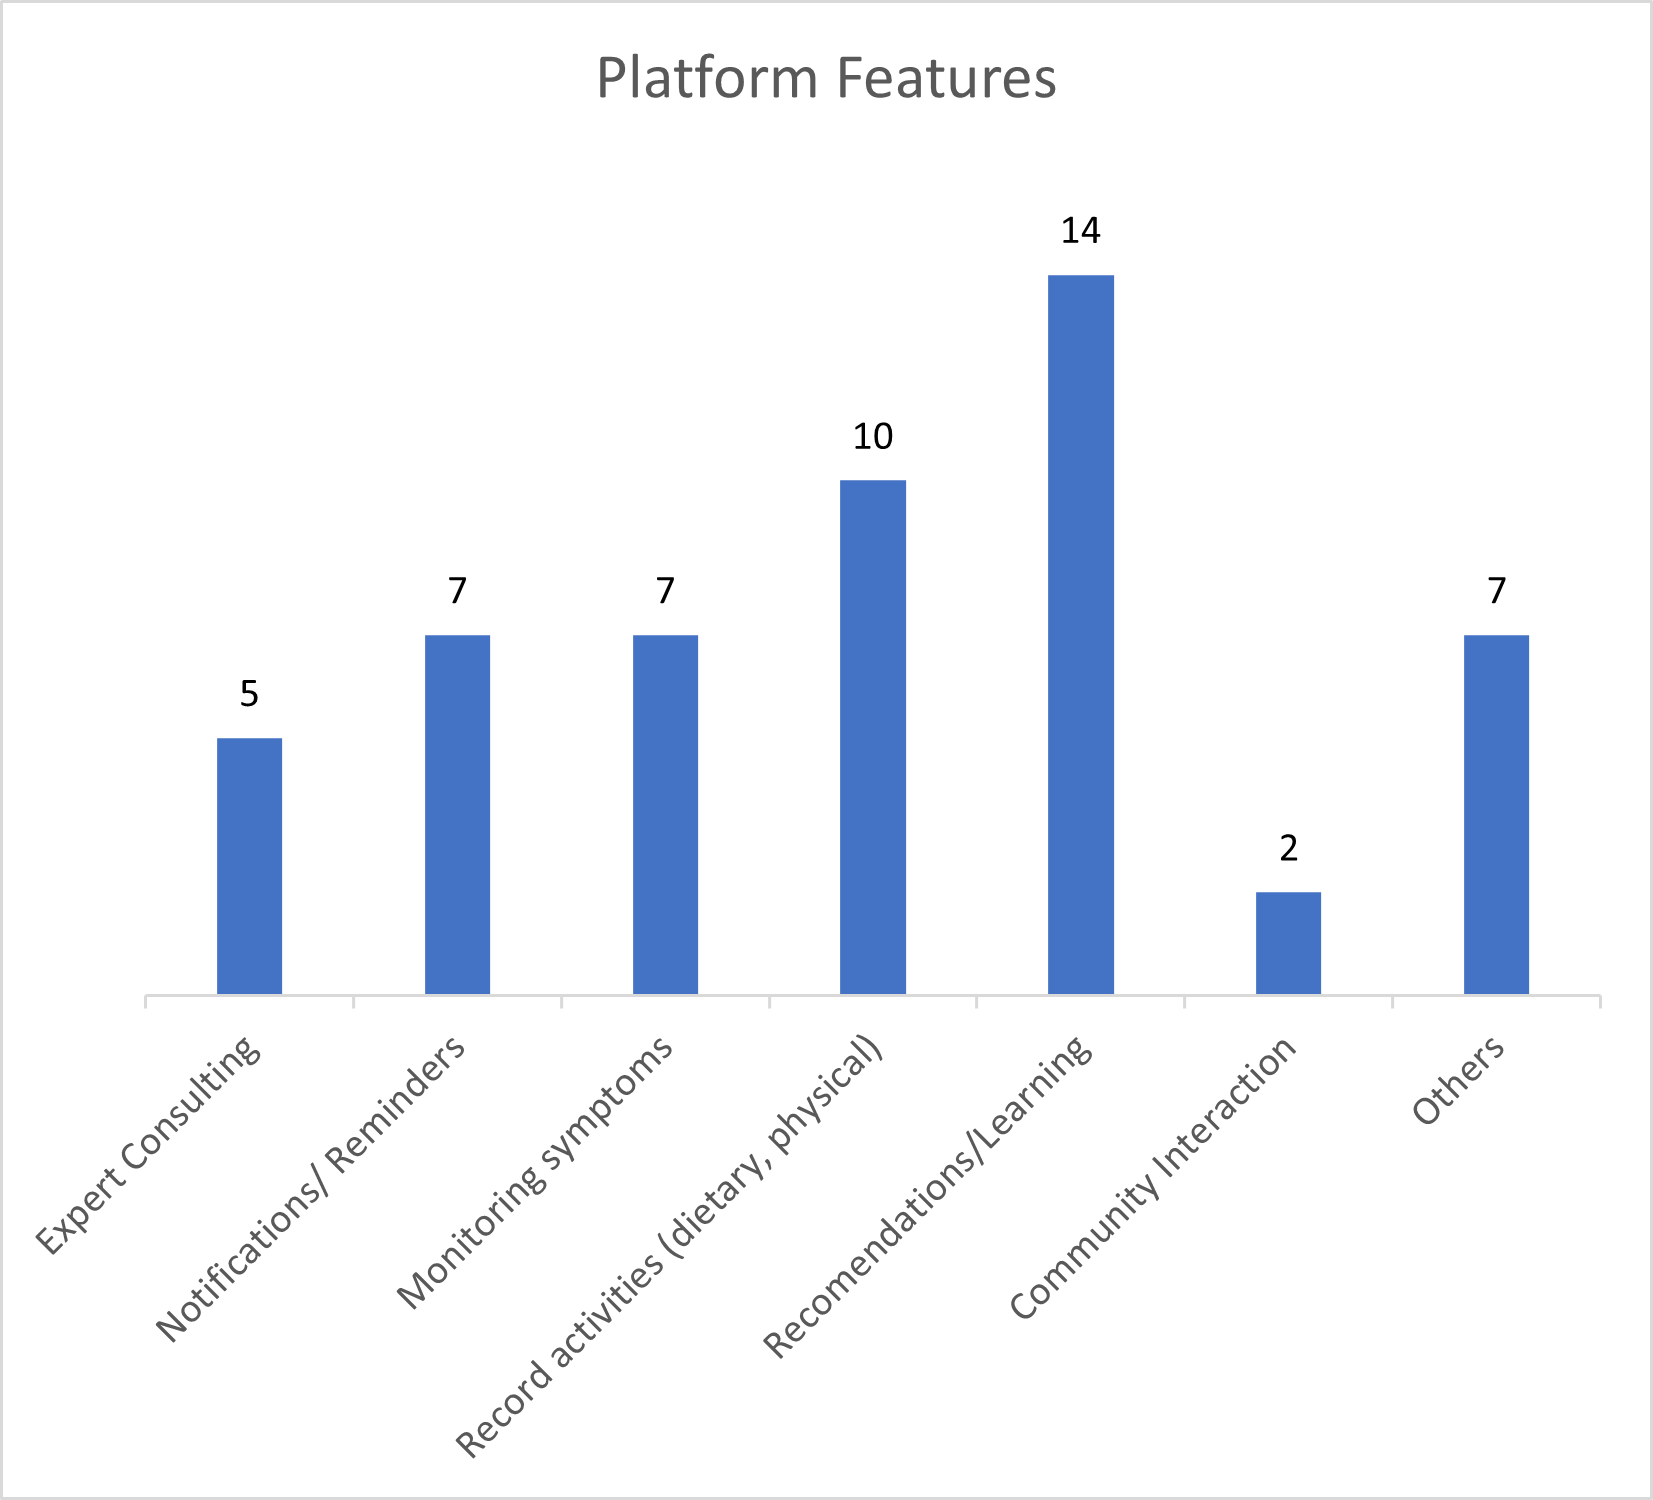
\includegraphics[width=0.45\textwidth]{charts/Features.png}
    \caption{Distribution of the features in the 16 studies.}
    \label{fig:features_chart}
\end{figure}

\subsubsection{Implementation}

Regarding the implementation of the platforms, we got that the majority of the platforms are mobile apps, as you can see in figure \ref{fig:platform_types}. On the other hand, figure \ref{fig:theoretical_frameworks} shows that there is no a popular theoretical framework to implement eHealth platforms for cancer patients.

\begin{figure}[h]
    \centering
    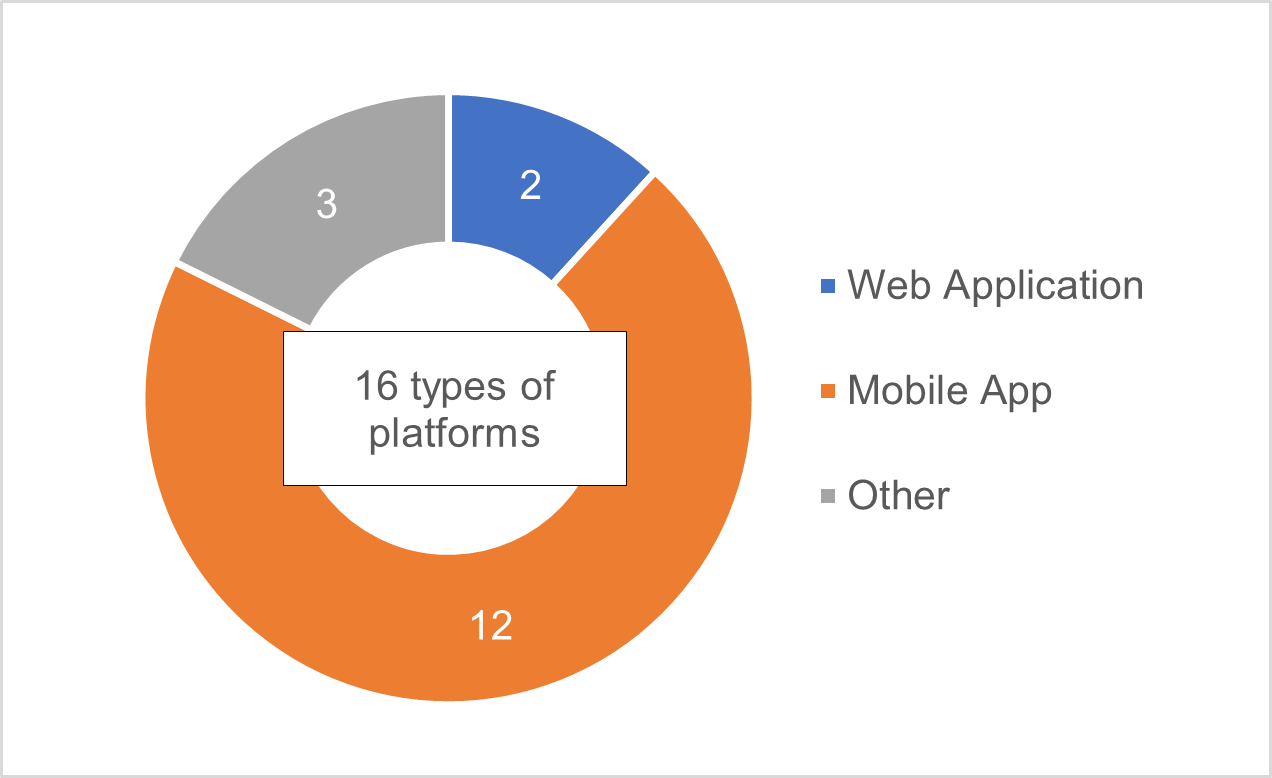
\includegraphics[width=0.30\textwidth]{charts/platform_types.png}
    \caption{Popularity of the platforms types.}
    \label{fig:platform_types}
\end{figure}


\begin{figure}[h]
    \centering
    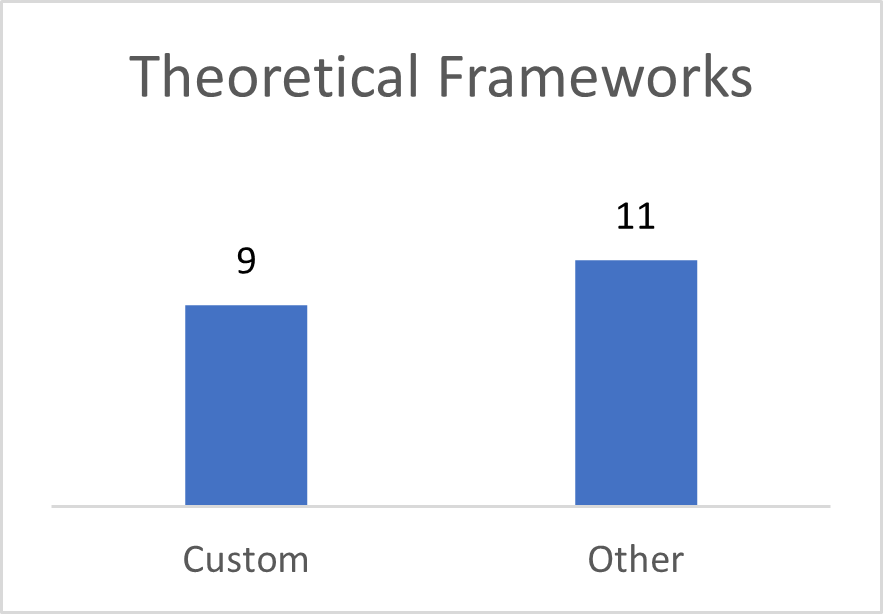
\includegraphics[width=0.30\textwidth]{charts/theoretical_frameworks.png}
    \caption{Reported theoretical frameworks used in the studies.}
    \label{fig:theoretical_frameworks}
\end{figure}

\subsubsection{Evaluation}

There was a considerable amount of information related to evaluations in this literature review. The most popular way to evaluate eHealth platforms is with questionnaires. Then, we found that some studies evaluated their platforms with experts reviews, interview with users, and users review. Figure \ref{fig:evaluations} summarizes the evaluations distribution.

\begin{figure}[h]
    \centering
    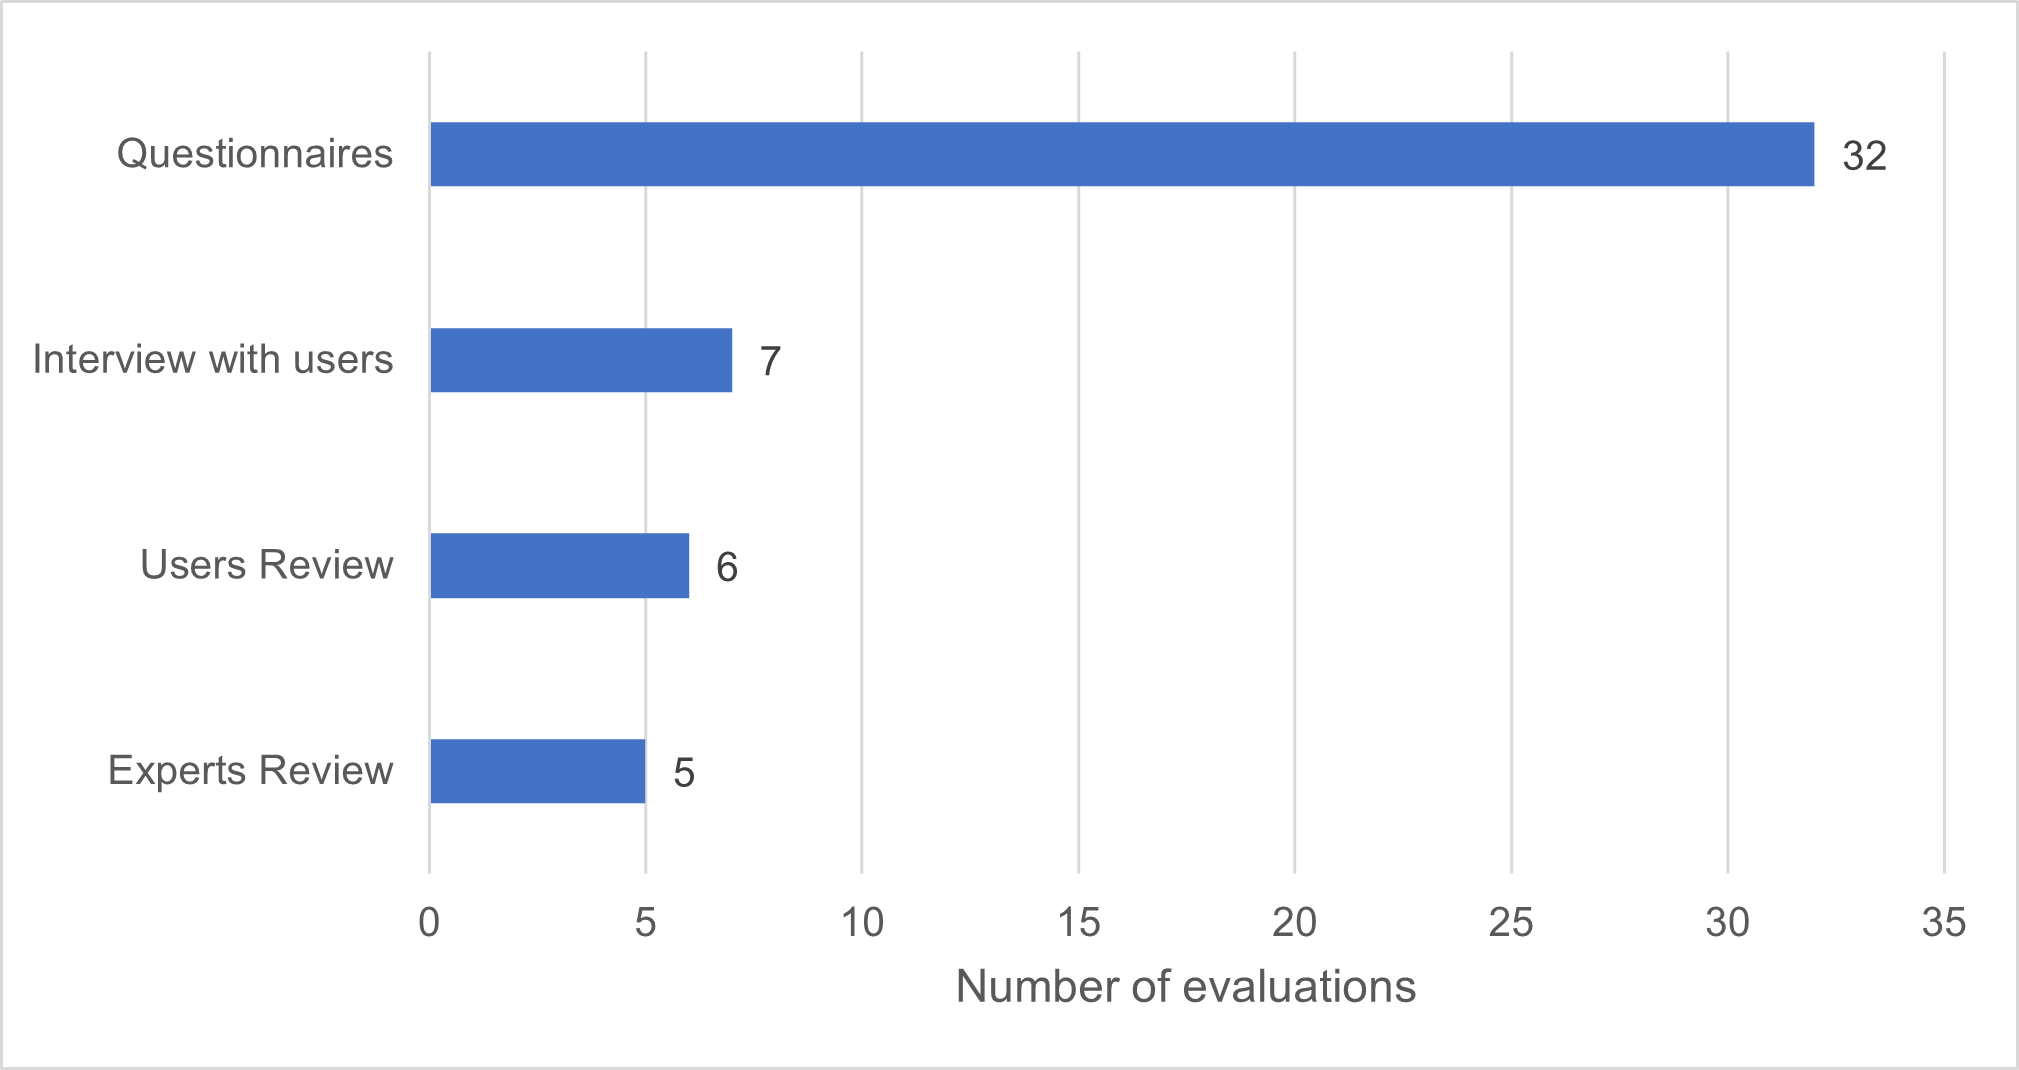
\includegraphics[width=0.40\textwidth]{charts/evaluations.png}
    \caption{Reported theoretical frameworks used in the studies.}
    \label{fig:evaluations}
\end{figure}

Due to there was a large volumes of information related to questionnaires, we decided to detail what kind of questionnaires were used, and their names. We found that there are 13 Health-Related Quality of Life questionnaires. This questionnaires measure the well-being of a patient \cite{Nahler2009}. Also, there are 9 functional assessment questionnaires. Functional assessment measures medical, physical, and mental health \cite{Sisto2018}. There are 4 eHealth questionnaires. We defined this category to group those questionnaires that measure how the platform works with the patients, note that this focus on the interaction between the patient and the platform. Finally, there are 5 usability questionnaires. Figure \ref{fig:questionnaires_types} summarizes the distribution.

\begin{figure}[h]
    \centering
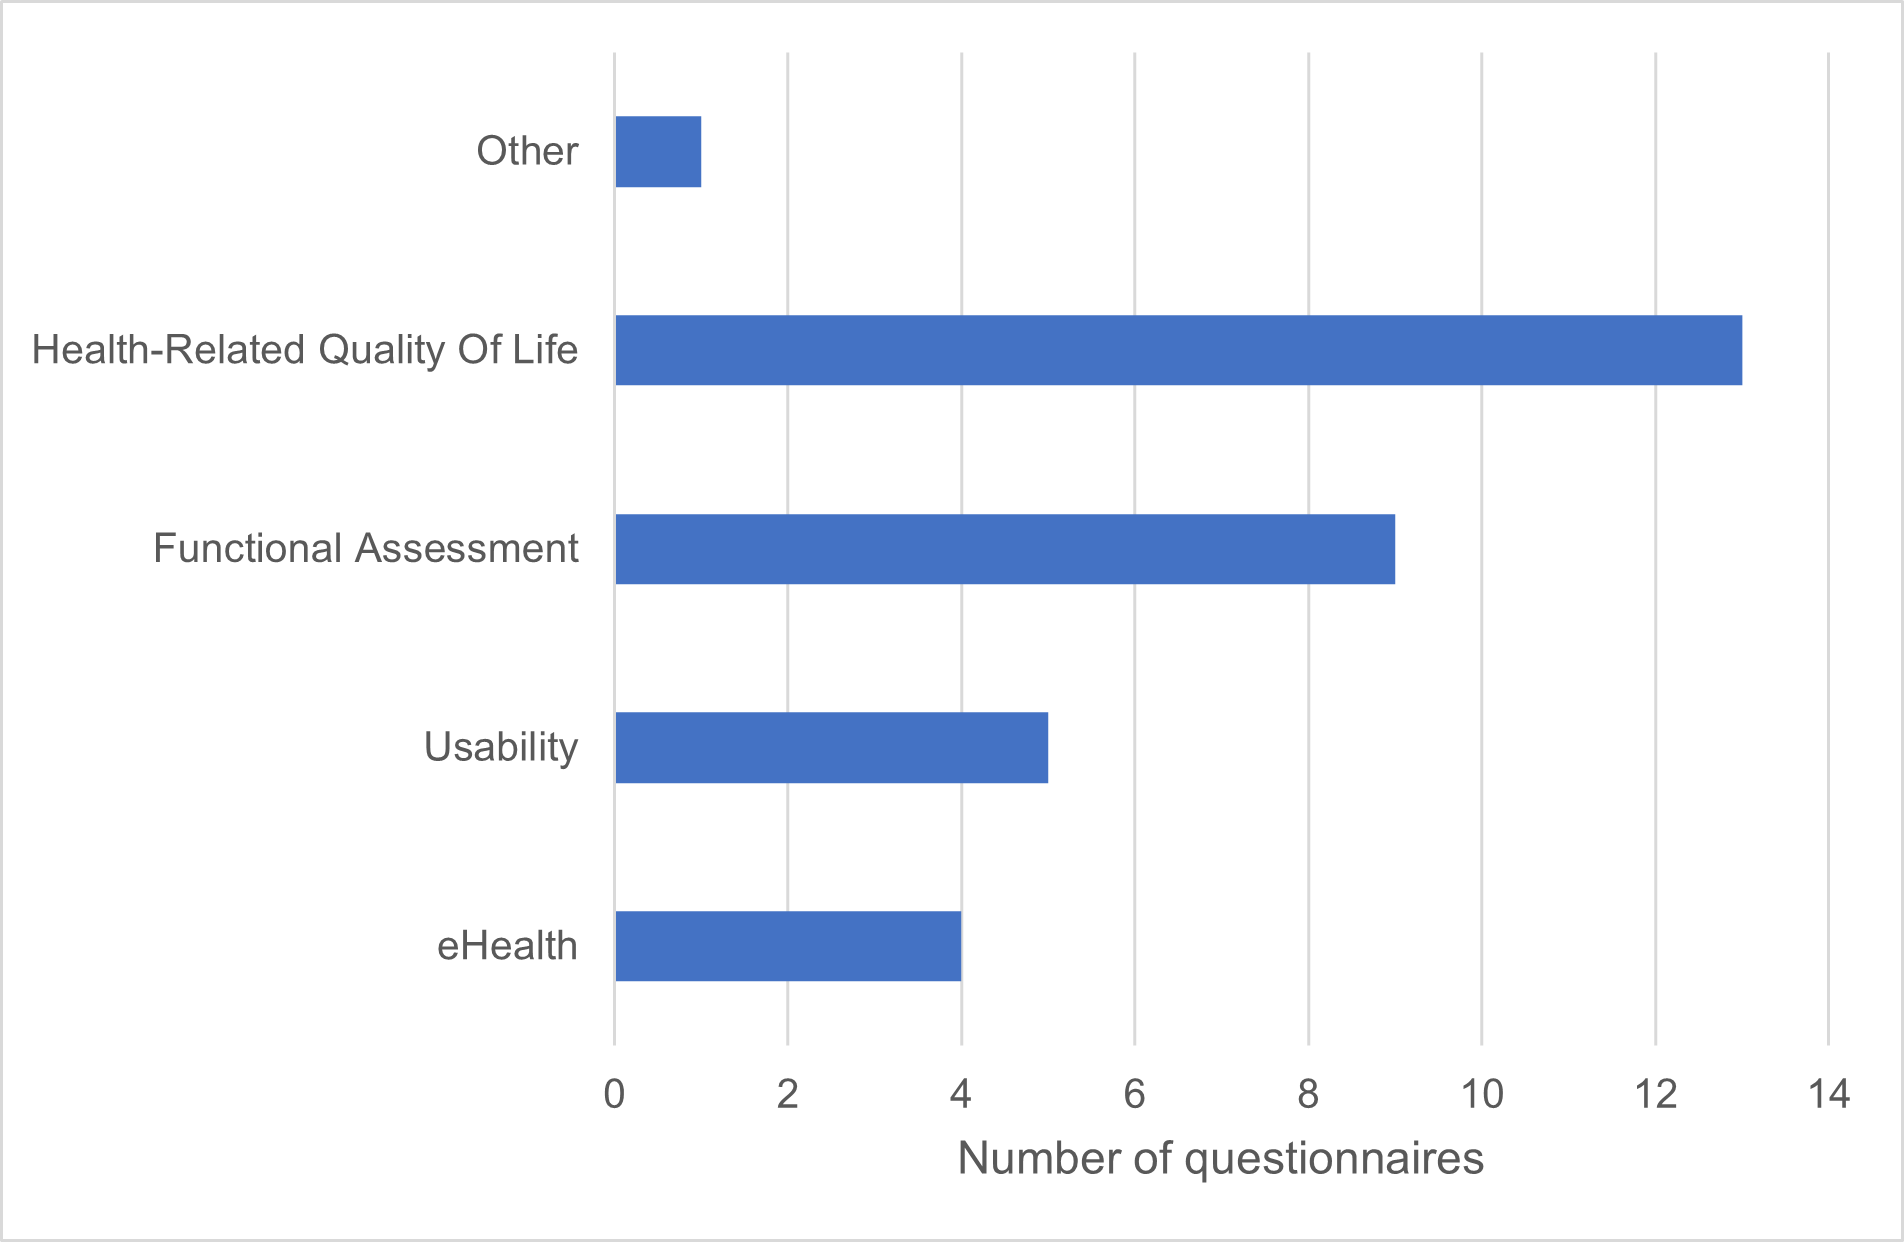
\includegraphics[width=0.40\textwidth]{charts/questionnaires_types.png}
    \caption{Types of questionnaires used to evaluate the eHealth platforms.}
    \label{fig:questionnaires_types}
\end{figure}

Finally, as you can see in figure \ref{fig:common_questionnaires}, we found some common questionnaires that were used. However, the majority are unique, therefore, we couldn't group them.

\begin{figure}[h]
    \centering
    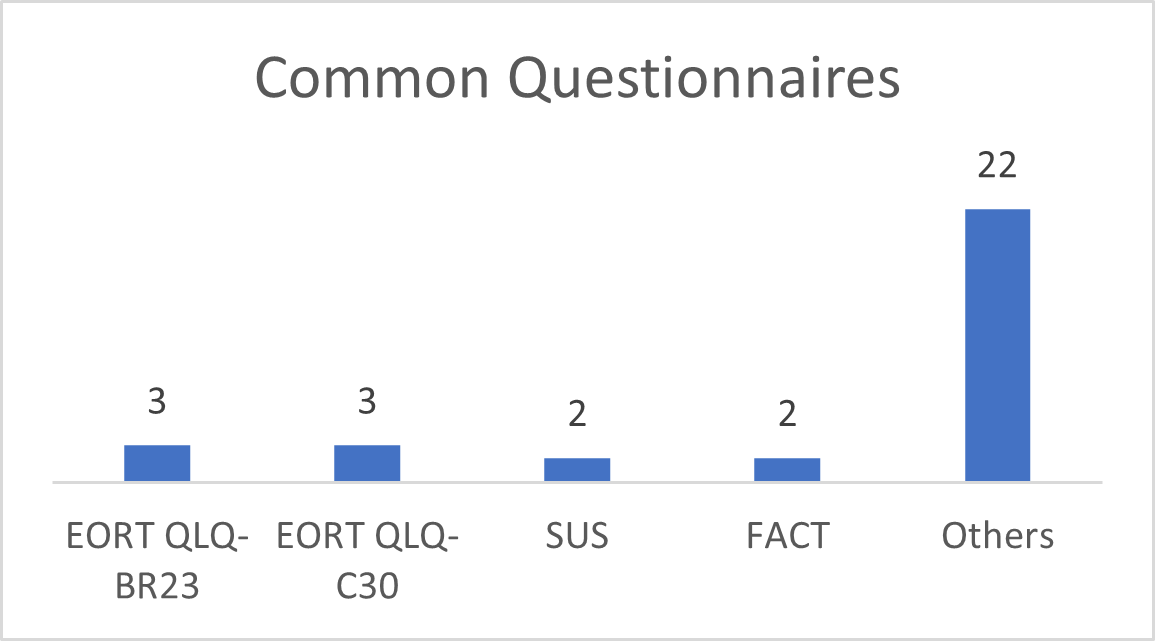
\includegraphics[width=0.40\textwidth]{charts/common_questionnaires.png}
    \caption{Grouped questionnaires names that were used to evaluate the eHealth platforms.}
    \label{fig:common_questionnaires}
\end{figure}

\subsubsection{Problems}
\label{subsubsection:problems}


Regarding the problems that were reported, we realized it's complicated to categorize. The reason is that every platform has their own needs and focus, despite we aimed for breast cancer platforms. Therefore, we only grouped the problems by usability and rehabilitation. Figure \ref{fig:reported_problems} shows the distribution of those problems.
\begin{figure}[h]
    \centering
    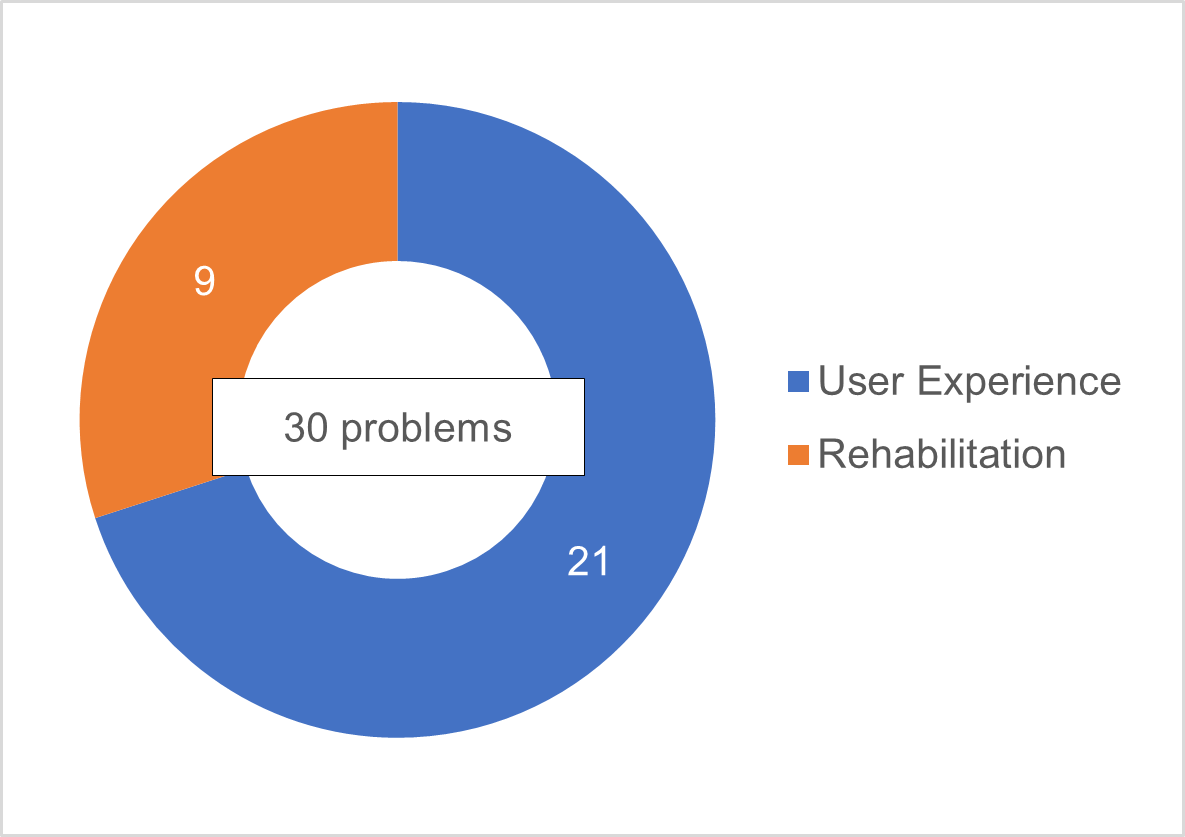
\includegraphics[width=0.30\textwidth]{charts/reported_problems.png}
    \caption{Amount of reported problems by usability and rehabilitation.}
    \label{fig:reported_problems}
\end{figure}


\section{Discussion}

In this section we will discuss three aspects related to the behavior of the studies and the data we gathered.

\subsection{Patients needs}

Most of the features reported in this literature review are related to the patients. Some of them are needed for doctors as well (like expert consulting), but overall patients are the main focus of the platform. Therefore, User-Centered-like methodologies are important to get a successful design. With these 16 studies, not every platform explicitly states they used the User-Centered Design, that's why we couldn't include it in the categorization.

In the same way, we can conclude that literature reviews cannot be the main way to start a design. As we saw on section \ref{subsubsection:problems}, every platform has their own needs. Therefore, researchers have to be careful with this approach, and think about the patients first.

\subsection{Technical information}

There is a clear lack of technical information to implement eHealth platform for breast cancer patients. We couldn't see a common theoretical framework across the studies.

Not enough information is available to make decisions. For example, what are the most useful frameworks to use? Is it good idea to implement hybrid mobile applications? What security concerns they have to mitigate? 

Therefore, there are no guidelines to follow. Some studies may use specific eHealth frameworks, but there is no standardization.

\subsection{Questionnaires}

Questionnaires are the most common way to evaluate eHealth platforms. We think the reasons are because it's cheaper in terms of money and time.

As well as the technical information, we couldn't find a standard questionnaire that were used across the studies. We only found questionnaires like EORT QLQ-BR23 and EORT QLQ-C30 that were used in three studies to measure Health-Related Quality Of Life.

Moreover, not even one standard questionnaire related to eHealth exclusively was found. Therefore, due the lack of standardization, some studies decided to use custom questionnaires, or general questionnaires to measure usability, such as SUS.

With these three aspects, we can conclude that our research question is answered partially. Questionnaires are the most common way to evaluate eHealth platforms. However, there is no available information related to how the platforms are implemented. We are aware that some of the studies used theoretical frameworks, but there isn't a popular one.

In our opinion, the lack of guidelines to design and implement eHealth platforms for breast cancer patients can affect the development of them. The possibility of repeating the same mistakes exists. Imagine if researchers would have access to eHealth heuristics to check the platform functionalities, unfortunately, that's not the case.

On the other hand, as we said before, even though the platforms aimed for breast cancer patients, they are not the same. Therefore, general guidelines can be somehow complicated to develop. However, we don't have enough data to have a solid conclusion about it.

\section{Conclusions}

The purpose of this literature review was to gathered the available data to understand how the platforms are characterized. We came out with four research questions to get the remarkable aspects of eHealth platforms. However, two of those questions were answered partially due to the lack of information reported.

Most of the studies focused on patients, instead of doctors, that's why there are more mobile apps. The platforms have the need to inform about the cancer, therapies, diets, exercises, among others. Questionnaires are the most popular way to evaluate platforms. There isn't a standard theoretical framework to develop eHealth platforms. Th problems reported in every platform are unique and depend on their needs.

Finally, we concluded that there is a need for guidelines or heuristics to check the validation of eHealth platforms. However, according to our analysis, heuristics for eHealth may be complicated due to the diversity a platform can have.


\bibliography{references}
\bibliographystyle{IEEEtran}

\end{document}